\section{Methods for Markov chains}
\label{m:sec:methods}

Having set out the processes, we turn to the techniques for extracting information
from them. The organising idea is the same throughout and is worth stating once
before it is applied: \emph{condition on one step, and solve the self-consistent
equation that results}. In discrete time the step is a generation and the equation
is a functional iteration; in continuous time the step is the first jump and the
equation is a differential one; for generating functions the step is an
infinitesimal interval and the equation is a partial differential equation. The
three settings look different and are the same gesture.

\subsection{Discrete-time methods}
\label{m:sec:dtmethods}

Discrete time is treated briefly here, for a specific reason. The techniques below
reduce every question about the Galton--Watson process of \cref{m:sec:gw} to a
question about the orbit of the quadratic map \cref{m:eq:SnIter}, and the method
that actually resolves that question --- the Koenigs linearisation, which
conjugates the map to a multiplication and turns the orbit into a geometric
sequence --- is the subject of \ChA. What follows is the machinery needed to reach
that point.

\subsubsection{First-step analysis}
\label{m:sec:firststep}

When the question is a hitting probability or a mean absorption time rather than a
full time course, conditioning on the first step replaces the evolution problem by
an algebraic one, because after that step the chain starts afresh from wherever it
landed.

\begin{proposition}[First-step principle]
\label{m:prop:firststep}
Let $\{X_n\}$ be a discrete-time Markov chain with transition matrix $P$ and
absorbing set $\mathcal A$, and let $h_i$ be the probability of ever reaching
$\mathcal A$ from state $i$. Then $h_i=1$ for $i\in\mathcal A$, and for every
transient $i$,
\begin{equation}
\label{m:eq:firststepdiscrete}
h_i = \sum_{j}P_{ij}\,h_j .
\end{equation}
The same conditioning applied to a continuous-time chain with generator $Q$ gives
\begin{equation}
\label{m:eq:firststep}
h_i = \sum_{j\neq i}\frac{q_{ij}}{q_i}\,h_j ,
\end{equation}
and the expected time to absorption satisfies
$k_i = 1/q_i + \sum_{j\neq i}(q_{ij}/q_i)k_j$.
\end{proposition}

\begin{proof}
Absorption occurs eventually if and only if it occurs from the state reached at the
first step; conditioning on that state and using the Markov property gives
\cref{m:eq:firststepdiscrete}. In continuous time the chain waits an
$\mathrm{Exp}(q_i)$ time and then, by \cref{m:prop:race}, jumps to $j$ with
probability $q_{ij}/q_i$ independently of the waiting time, which gives
\cref{m:eq:firststep}; adding the expected holding time $1/q_i$ to the same
decomposition gives the equation for $k_i$.
\end{proof}

Note what \cref{m:eq:firststep} does not contain: the holding times have vanished.
Hitting \emph{probabilities} for a continuous-time chain depend only on the
embedded jump chain of \cref{m:sec:randomwalk}, not on the rates themselves. Mean
hitting times do depend on the rates, which is why $1/q_i$ appears in the companion
system. The gambler's-ruin formula \cref{m:eq:gamblersruin} is the two-term instance
of \cref{m:eq:firststepdiscrete}, and \cref{m:sec:hitting} applies it to the
birth--death process.

For a branching process the first-step decomposition produces something better than
a linear system. Because the offspring of the founder generate independent
subpopulations, conditioning on the first generation gives a \emph{fixed-point
equation}: the ultimate extinction probability $s$ from a single individual
satisfies
\begin{equation}
\label{m:eq:extinctionfixedpoint}
s = \phi(s) ,
\end{equation}
$\phi$ being the offspring generating function. That is the whole content of
\cref{m:sec:extinction}.

\subsubsection{Generating functions}
\label{m:sec:pgfmethod}

For a \rv{} $X$ taking values in $\{0,1,2,\dots\}$ with $p_k=\pr{X=k}$, the
\pgf{} is
\begin{equation}
\label{m:eq:pgfdef}
\phi(z) = \ex{z^X} = \sum_{k=0}^{\infty}p_kz^k ,
\end{equation}
convergent at least for $|z|\le1$. The series determines the distribution, since
$p_k=\phi^{(k)}(0)/k!$, and moments are read off at $z=1$:
\begin{equation}
\label{m:eq:pgfmoments}
\phi(1)=1,
\qquad
\phi'(1) = \ex{X},
\qquad
\phi''(1) = \ex{X(X-1)} .
\end{equation}
Two structural properties do most of the work. If $X$ and $Y$ are independent then
$\phi_{X+Y}=\phi_X\phi_Y$, so sums become products. And if $N$ is an independent
count with \pgf{} $\psi$, the random sum $X_1+\dots+X_N$ of independent copies of
$X$ has \pgf{} $\psi\circ\phi$: \emph{composition} of generating functions
corresponds to compounding, which is exactly the structure of
\cref{m:eq:gwrecursion} and hence the source of \cref{m:eq:gwcomposition}.

For a pair of counts the definition extends to
\begin{equation}
\label{m:eq:pgfbivariate}
G(x,y) = \ex{x^Xy^Y} = \sum_i\sum_j\pr{X=i,\ Y=j}\,x^iy^j ,
\end{equation}
with marginals recovered by setting the other variable to one; the absorption
models of \cref{m:sec:moc} need this form, and \cref{m:app:extract} records how to
invert it. The same construction with $n$ arguments handles vector-valued states
and is the prepared ground for the multi-type models of later chapters; it is not
developed here.

\subsubsection{Functional iteration}
\label{m:sec:iteration}

Applying \cref{m:eq:gwcomposition} repeatedly, the generating function of $Z_n$ is
the $n$-fold composite $\phi_n=\phi^{\circ n}$, and every question about the
Galton--Watson process becomes a question about iterating a single map. For the
binary law \cref{m:eq:pgfbinary} this is the quadratic recursion \cref{m:eq:SnIter}
for the survival probability, obtained by evaluating at $z=0$ and taking
complements.

\begin{proposition}[Certainty of extinction]
\label{m:sec:extinction}
For the binary Galton--Watson process, $S_n$ decreases to a limit $S_\infty$ which
is a fixed point of $S\mapsto2pS-pS^2$. Consequently
\begin{equation}
\label{m:eq:Sinfty}
S_\infty =
\begin{cases}
0, & p\le\tfrac12,\\[4pt]
\dfrac{2p-1}{p}, & p>\tfrac12 .
\end{cases}
\end{equation}
\end{proposition}

\begin{proof}
A population cannot return from extinction, so $u_n$ is non-decreasing and bounded
by $1$; equivalently $S_n$ is non-increasing and bounded below by $0$, so it
converges, and its limit must be a fixed point. Setting $S=2pS-pS^2$ gives
$pS\bigl(S+\tfrac1p-2\bigr)=0$, with roots $S=0$ and $S=2-1/p=(2p-1)/p$. For
$p<\tfrac12$ the second root is negative and carries no probabilistic meaning, so
the only admissible limit is $0$; at $p=\tfrac12$ the two roots collide there. For
$p>\tfrac12$ the origin turns repelling and the positive root is attained.
\end{proof}

\Cref{m:fig:phase_transition} shows the transition together with the change of
stability that produces it. The qualitative picture is the standard one for a
transcritical bifurcation, and it is worth noticing that the whole of
\cref{m:sec:extinction} is a statement about the fixed points of a quadratic map:
the probabilistic content has been fully converted into dynamics.

\begin{figure}[htbp]
    \centering
    \begin{subfigure}[b]{0.31\textwidth}
        \centering
        \begin{tikzpicture}
            \begin{axis}[ch2plotstyle]
                \addplot[blue, thick] {2*0.3*x - 0.3*x^2};
                \addplot[black!45, dashed] {x};
                \addplot[only marks, mark=*, red, mark size=1.6pt] coordinates {(0,0)};
            \end{axis}
        \end{tikzpicture}
        \caption{Subcritical ($p = 0.3$)}
    \end{subfigure}
    \hfill
    \begin{subfigure}[b]{0.31\textwidth}
        \centering
        \begin{tikzpicture}
            \begin{axis}[ch2plotstyle]
                \addplot[blue, thick] {2*0.5*x - 0.5*x^2};
                \addplot[black!45, dashed] {x};
                \addplot[only marks, mark=*, red, mark size=1.6pt] coordinates {(0,0)};
            \end{axis}
        \end{tikzpicture}
        \caption{Critical ($p = 0.5$)}
    \end{subfigure}
    \hfill
    \begin{subfigure}[b]{0.31\textwidth}
        \centering
        \begin{tikzpicture}
            \begin{axis}[ch2plotstyle]
                \addplot[blue, thick] {2*0.74*x - 0.74*x^2};
                \addplot[black!45, dashed] {x};
                \addplot[only marks, mark=*, red, mark size=1.6pt] coordinates {(0,0) (0.64865,0.64865)};
            \end{axis}
        \end{tikzpicture}
        \caption{Supercritical ($p = 0.74$)}
    \end{subfigure}

    \vspace{10pt}
    \begin{subfigure}[b]{0.55\textwidth}
    \centering
    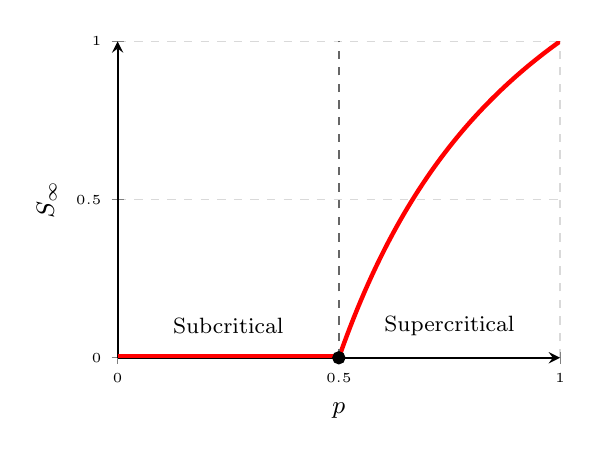
\begin{tikzpicture}
        \begin{axis}[
            width=7.2cm, height=5.6cm,
            axis lines=left,
            xlabel={$p$}, ylabel={$S_\infty$},
            xmin=0, xmax=1, ymin=0, ymax=1,
            xtick={0,0.5,1}, ytick={0,0.5,1},
            grid=major, grid style={dashed, gray!30}, thick,
            label style={font=\small}, tick label style={font=\tiny}
        ]
            \addplot[red, ultra thick, domain=0:0.5] {0.004};
            \addplot[red, ultra thick, domain=0.5:1, samples=120] {(2*x-1)/x};
            \draw[dashed, black!60] (axis cs:0.5,0) -- (axis cs:0.5,1);
            \node[font=\footnotesize] at (axis cs:0.25, 0.10) {Subcritical};
            \node[font=\footnotesize] at (axis cs:0.75, 0.10) {Supercritical};
            \addplot[only marks, mark=*, mark size=2pt, black] coordinates {(0.5,0)};
        \end{axis}
    \end{tikzpicture}
    \caption{The transition in $S_\infty$}
    \end{subfigure}

    \caption{Fixed points of the survival recursion \cref{m:eq:SnIter}. Panels
    (a)--(c) show the map $S\mapsto 2pS-pS^2$ (blue) against the diagonal (dashed),
    with the fixed points marked in red. Below and at criticality the origin is the
    only fixed point in $[0,1]$ and it is attracting, so extinction is certain; at
    $p=\tfrac12$ the map is tangent to the diagonal there. For $p>\tfrac12$ the
    origin turns repelling and a stable positive fixed point $S_\infty=(2p-1)/p$
    separates from it, traced in panel~(d). The survival probability is identically
    zero below the critical point and rises continuously above it.}
    \label{m:fig:phase_transition}
\end{figure}

\subsubsection{Where the discrete-time methods run out}
\label{m:sec:dtlimit}

Fixed points are the easy part. The hard question is not \emph{whether} $S_n\to0$
in the subcritical case but \emph{how}, and there the elementary methods stop.
Since the quadratic term in \cref{m:eq:SnIter} becomes negligible once $S_n$ is
small, the decay is asymptotically geometric with ratio $2p$. The ratio is
immediate; the constant standing in front of it is not,
\begin{equation}
\label{m:eq:Apdef}
A(p) = \lim_{n\to\infty}\frac{S_n}{(2p)^n},
\qquad\text{so that}\qquad
S_n\sim A(p)\,(2p)^n .
\end{equation}
We call $A(p)$ the \emph{amplitude} of the decay, and use it under that name
throughout. The amplitude accumulates every early nonlinear correction made before
the recursion attenuates to $S_{n+1}\approx2pS_n$, which is precisely what the
late-time behaviour has already forgotten. No argument confined to late generations
can therefore produce it, and no elementary formula for it is known.

The technique that addresses this is a change of coordinate. Substituting
$S_n=2w_n$ and $r=2p$ turns \cref{m:eq:SnIter} into the logistic map
$w_{n+1}=rw_n(1-w_n)$, and one asks for a coordinate in which that map becomes
multiplication by $r$ --- a solution $\psi_r$ of the Schröder equation
$\psi_r(f_r(z))=r\psi_r(z)$, the Koenigs linearising function. In that coordinate
the orbit is exactly geometric and its amplitude can be read off. \ChAcap{} carries
this out, identifies $A(p)$ with twice a value of $\psi_{2p}$, and proves that
$\psi_r$ is hypertranscendental for every $r$ in the subcritical window --- which
is why the elementary methods of this subsection could not have succeeded. Nothing
further about $A(p)$ is developed here; it is used below as a named object.

\subsection{Continuous-time methods}
\label{m:sec:ctmethods}

The continuous-time methods carry the technical weight of this chapter. They are
presented on the linear birth--death process of \cref{m:sec:bd} throughout, both
because it is the process the thesis actually uses and because it is simple enough
that each method can be seen working rather than merely stated.

\subsubsection{Forward and backward equations}
\label{m:sec:backward}

Differentiating the Chapman--Kolmogorov identity
$p_{ij}(t+\Delta t)=\sum_kp_{ik}(t)p_{kj}(\Delta t)$ at $\Delta t=0$ gives the
\emph{forward} equations,
\begin{equation}
\label{m:eq:forward}
\ddt{p_{ij}(t)} = \sum_kp_{ik}(t)\,q_{kj},
\qquad\text{that is}\qquad
\dda{P}{t} = PQ ,
\end{equation}
which condition on the last jump before time $t$. Differentiating in the other slot
gives the \emph{backward} equations,
\begin{equation}
\label{m:eq:backwardeq}
\dda{P}{t} = QP ,
\end{equation}
which condition on the first jump after time $0$ --- first-step analysis in
differential form. The two carry the same information but suit different questions:
forward equations track the distribution as it spreads, backward equations track a
functional of the whole future and are the natural setting for absorption
probabilities and for the generating function of a branching process.

Written out for a fixed initial state, with $p_j(t)$ the probability of occupying
state $j$, \cref{m:eq:forward} becomes the \emph{master equation}
\begin{equation}
\label{m:eq:master}
\ddt{p_j(t)} = \sum_{k\neq j}q_{kj}\,p_k(t) - q_j\,p_j(t) :
\end{equation}
probability flows into $j$ from every state that can reach it and out of $j$ at
total rate $q_j$. Every model in this thesis is specified by writing down
\cref{m:eq:infinitesimal} and reading off \cref{m:eq:master}.

For the birth--death rates \cref{m:eq:bdrates} the master equation is
\begin{equation}
\label{m:eq:bdmaster}
\ddt{p_n(t)} = \lambda(n-1)p_{n-1}(t) + \mu(n+1)p_{n+1}(t) - (\lambda+\mu)n\,p_n(t),
\end{equation}
an infinite coupled system, and on its own it is not much use. The step that makes
it tractable is to collapse it into a single equation for a generating function.
Multiply \cref{m:eq:bdmaster} by $z^n$, sum over $n\ge0$, and shift indices so that
every sum is again of the form \cref{m:eq:pgfdef}; the factors of $n$ produced by
the linear rates become derivatives $\partial_z$, and the three terms become
$\lambda z^2\partial_zG$, $\mu\partial_zG$ and $-(\lambda+\mu)z\partial_zG$. Hence
\begin{equation}
\label{m:eq:bdpde}
\pddt{G} = \bigl(\lambda z^2-(\lambda+\mu)z+\mu\bigr)\pdd{G}{z}
= (\lambda z-\mu)(z-1)\pdd{G}{z},
\qquad
G(z,0)=z^N ,
\end{equation}
for a process started from $N$ individuals. This is the template for every
generating-function calculation in this thesis. Note where the linearity of the
rates was used: it is what makes the coefficient a polynomial in $z$ and the
equation first order, and hence what puts it within reach of
\cref{m:sec:moc}. The quadratic coefficient factorises with roots $z=1$ and
$z=\mu/\lambda$, and the same factorisation reappears in
\cref{m:app:absbirthdeath}.

Solving \cref{m:eq:bdpde} along its characteristics gives the classical result of
Kendall \cite{Kendall1948},
\begin{equation}
\label{m:eq:bdsolution}
G(z,t) = \lrb{\frac{\mu(1-z)-(\mu-\lambda z)\ee^{-(\lambda-\mu)t}}
{\lambda(1-z)-(\mu-\lambda z)\ee^{-(\lambda-\mu)t}}}^{\!N},
\qquad\lambda\neq\mu .
\end{equation}
Everything in the next four subsections is extracted from this one formula, or
obtained more cheaply by a route that \cref{m:eq:bdsolution} then confirms.

\subsubsection{Mean population size}
\label{m:sec:mean}

Differentiating \cref{m:eq:bdsolution} at $z=1$ is possible and unpleasant. It is
quicker to take the mean of the master equation directly: multiplying
\cref{m:eq:bdmaster} by $n$ and summing, the terms telescope to
\begin{equation}
\label{m:eq:meanode}
\ddt{}\ex{X_t} = (\lambda-\mu)\ex{X_t},
\qquad
\ex{X_0}=N,
\end{equation}
whence
\begin{equation}
\label{m:eq:bdmean}
\ex{X_t} = N\ee^{(\lambda-\mu)t} .
\end{equation}
The mean obeys a closed equation --- exactly the deterministic rate equation one
would have written down without any probability at all --- and this is a special
feature of \emph{linear} rates. It is also the reason the mean is uninformative
here: \cref{m:eq:bdmean} is the same whether the process is a near-certain
extinction with a rare enormous excursion or a steady moderate growth, and
distinguishing those is the entire problem.

\subsubsection{Variance and higher moments}
\label{m:sec:variance}

The second moment is obtained the same way. Multiplying \cref{m:eq:bdmaster} by
$n^2$ and summing gives
\begin{equation}
\label{m:eq:secondmomentode}
\ddt{}\ex{X_t^2} = 2(\lambda-\mu)\ex{X_t^2} + (\lambda+\mu)\ex{X_t},
\end{equation}
a linear equation driven by the known mean \cref{m:eq:bdmean}. Solving with the
integrating factor $\ee^{-2(\lambda-\mu)t}$ and subtracting $\ex{X_t}^2$ gives, for
$\lambda\neq\mu$,
\begin{equation}
\label{m:eq:bdvariance}
\var{X_t} = N\,\frac{\lambda+\mu}{\lambda-\mu}\,
\ee^{(\lambda-\mu)t}\lrb{\ee^{(\lambda-\mu)t}-1},
\end{equation}
and in the critical case $\lambda=\mu$ the limit is $\var{X_t}=2N\lambda t$. Two
readings are worth recording. In the subcritical case $\lambda<\mu$ both mean and
variance decay, but the variance decays more slowly --- the coefficient of
variation grows, and the process becomes relatively \emph{more} random as it dies.
At criticality the mean is constant and the variance grows without bound, which is
the analytic signature of the heavy tail examined in \cref{m:app:criticalgw}.

The pattern generalises. Multiplying the master equation by $n^{\varrho}$ produces
an equation for the $\varrho$th moment driven by the lower ones, so the moments can
be found recursively without ever solving \cref{m:eq:bdpde}. Equivalently,
differentiating \cref{m:eq:bdpde} repeatedly at $z=1$ and using
\cref{m:eq:pgfmoments} gives the same hierarchy; the hierarchy closes at each level
precisely because the rates are linear. For a process with nonlinear rates the
moment equations do not close, and the generating-function route of
\cref{m:sec:moc} becomes not merely convenient but necessary.

\subsubsection{Hitting probabilities}
\label{m:sec:hitting}

Hitting probabilities are where first-step analysis earns its place, because they
require no time-dependent solution at all. By \cref{m:prop:firststep} the
probability $h_i$ of ever reaching a target set from state $i$ satisfies
\cref{m:eq:firststep}, which involves only the ratios $q_{ij}/q_i$ --- the embedded
jump chain. For the birth--death rates \cref{m:eq:bdrates} those ratios are
independent of the state,
\begin{equation}
\label{m:eq:bdjumpratios}
\frac{q_{n,n+1}}{q_n} = \frac{\lambda n}{(\lambda+\mu)n} = \frac{\lambda}{\lambda+\mu},
\qquad
\frac{q_{n,n-1}}{q_n} = \frac{\mu}{\lambda+\mu},
\end{equation}
so the embedded chain is the simple random walk of \cref{m:sec:randomwalk} with
$q=\lambda/(\lambda+\mu)$, and \cref{m:eq:gamblersruin} answers the question
immediately. With absorbing barriers at $0$ and $M$, the probability of reaching
$M$ before extinction, starting from $i$ individuals, is
\begin{equation}
\label{m:eq:bdruin}
h_i = \frac{1-(\mu/\lambda)^i}{1-(\mu/\lambda)^M}
\qquad(\lambda\neq\mu),
\qquad
h_i = \frac{i}{M}
\qquad(\lambda=\mu),
\end{equation}
since $\theta = (1-q)/q = \mu/\lambda$. Letting $M\to\infty$ gives the probability
of unbounded growth, $1-(\mu/\lambda)^i$ when $\lambda>\mu$ and $0$ otherwise,
which is the complement of the extinction probability found independently in
\cref{m:sec:extinctionprob}. The two routes agreeing is a useful check on both.

Mean hitting times behave differently and the difference is instructive. They
depend on the rates and not merely on their ratios, and at criticality
$\lambda=\mu$ the mean time to absorption is infinite even though absorption is
certain --- the continuous-time counterpart of the phenomenon derived in full in
\cref{m:app:criticalgw}.

\subsubsection{Extinction probabilities}
\label{m:sec:extinctionprob}

Extinction by time $t$ is the event $X_t=0$, so its probability is the generating
function evaluated at the origin: $p_0(t)=G(0,t)$. From \cref{m:eq:bdsolution},
\begin{equation}
\label{m:eq:p0t}
p_0(t) =
\begin{cases}
\displaystyle\lrb{\frac{\mu-\mu\ee^{(\mu-\lambda)t}}{\lambda-\mu\ee^{(\mu-\lambda)t}}}^{\!N},
& \lambda\neq\mu,\\[14pt]
\displaystyle\lrb{\frac{\lambda t}{1+\lambda t}}^{\!N},
& \lambda=\mu,
\end{cases}
\end{equation}
the critical case following by taking $\mu\to\lambda$ in the first line. Letting
$t\to\infty$ recovers the threshold: extinction is certain when $\lambda\le\mu$ and
occurs with probability $(\mu/\lambda)^N$ when $\lambda>\mu$, which is the
complement of \cref{m:eq:bdruin} with $M\to\infty$, as it must be.

\Cref{m:fig:extinction} plots \cref{m:eq:p0t}, alongside the law it leaves behind.

\begin{figure}[ht]
\centering

\includegraphics[width=0.98\textwidth]{extinction_and_law.pdf}
\caption{(a) The extinction probability \cref{m:eq:p0t} against time, with $\mu=1$
and $\lambda=0.6,\,1,\,1.4$; solid curves start from $N=1$, dashed from $N=5$.
Below and at criticality every curve climbs to one, however large the founding
cohort; above it the curves level off at $(\mu/\lambda)^N$, marked dotted for
$N=1$, and a larger cohort buys a permanently smaller extinction probability rather
than merely a delay.
(b) The critical case in detail, from one founder: the law of $X_t$ on the positive
states at $t=1,3,10$, on a logarithmic scale. Absorbing mass accumulates at zero
--- $p_0$ rises from $0.50$ to $0.91$ --- while the surviving tail flattens and
stretches. The mean is exactly $1$ at all three times. Neither the growing chance
of extinction nor the lengthening tail is visible in that number, which is the
sense in which the mean of \cref{m:eq:bdmean} answers the wrong question.}
\label{m:fig:extinction}
\end{figure}

The survival probability is $S^{(N)}(t)=1-p_0(t)$, and for a single founder,
$N=1$, \cref{m:eq:p0t} rearranges to
\begin{equation}
\label{m:eq:ctsS}
S(t) = \frac{\lambda-\mu}{\lambda-\mu\ee^{(\mu-\lambda)t}}
= \frac{\mu-\lambda}{\mu}\,\ee^{-(\mu-\lambda)t}
\lrb{1-\frac{\lambda}{\mu}\ee^{-(\mu-\lambda)t}}^{-1}
\;\sim\;\frac{\mu-\lambda}{\mu}\,\ee^{-(\mu-\lambda)t}
\end{equation}
as $t\to\infty$, in the subcritical case $\mu>\lambda$. The last form is the one
that matters below: the survival probability decays exponentially with a definite
\emph{amplitude} $(\mu-\lambda)/\mu$, and because \cref{m:eq:ctsS} is elementary at
every $t$, that amplitude can simply be read off. Contrast \cref{m:eq:Apdef}, where
the analogous amplitude is available only as a limit.

\subsubsection{Conditional means}
\label{m:sec:condmeans}

Absorption is often inevitable --- for $\lambda<\mu$, and for the whole subcritical
branching range --- and yet a process on its way to absorption need not be
featureless. In many cases it settles, long before it is absorbed, into a
distribution that no longer changes with time: a distribution describing the
population conditional on its not yet having been absorbed. The phenomenon is
\emph{quasi-stationarity} and the limit is the Yaglom limit \cite{Yaglom1947};
modern accounts are Méléard and Villemonais \cite{Meleard2012} and Collet,
Martínez and San Martín \cite{Collet2013}.

\begin{definition}[Quasi-stationary and Yaglom laws]
\label{m:def:qsd}
Let $\{X_t\}$ be a Markov process with absorbing state $0$. A probability
distribution $\nu$ on the non-absorbing states is \emph{quasi-stationary} if
$\pr{X_t=j\mid X_t\neq0}=\nu_j$ for all $t\ge0$ and $j\neq0$ whenever
$X_0\sim\nu$. If, from a specified initial state,
$\pr{X_t=j\mid X_t\neq0}\to\nu_j$, then $\nu$ is the corresponding \emph{Yaglom
limit}.
\end{definition}

Existence of the Yaglom limit for the processes used here is classical, from Yaglom
\cite{Yaglom1947} with modern treatments in \cite{Harris1963,Athreya1972,Meleard2012},
and is taken from that literature rather than re-proved. What is computed below is
the limiting conditional mean, explicitly, in both time scales. The distinction
matters: convergence of moments is consistent with the Yaglom theorem but does not
on its own establish convergence of the full conditional law.

\paragraph{The continuous-time constant.}
Since $X_t=0$ contributes nothing to its own expectation,
\begin{equation}
\label{m:eq:condit}
\ex{X_t\mid X_t>0} = \frac{\ex{X_t}}{S^{(N)}(t)} ,
\end{equation}
and for $N=1$ substituting \cref{m:eq:bdmean} and \cref{m:eq:ctsS} gives, exactly,
\begin{equation}
\label{m:eq:ctscondmean}
\ex{X_t\mid X_t>0}
= \frac{\ee^{(\lambda-\mu)t}\lrb{\lambda-\mu\ee^{(\mu-\lambda)t}}}{\lambda-\mu}
= \frac{\lambda\ee^{(\lambda-\mu)t}-\mu}{\lambda-\mu} .
\end{equation}
For $\mu>\lambda$ the exponential decays and the limit is a constant,
\begin{equation}
\label{m:eq:ctsqsmean}
\lim_{t\to\infty}\ex{X_t\mid X_t>0} = \frac{\mu}{\mu-\lambda}
= \frac{1}{1-\lambda/\mu}
=: \frac{1}{\Ac} ,
\end{equation}
the reciprocal of the amplitude identified in \cref{m:eq:ctsS}. To compare this with
the discrete-generation model the two parametrisations must be matched, and
\cref{m:prop:race} is what matches them: the probability that the birth clock wins
is $p=\lambda/(\lambda+\mu)$, so $\lambda/\mu=p/(1-p)$, and
\begin{equation}
\label{m:eq:Acts}
\Ac(p) = \frac{1-2p}{1-p} = \frac{2\varepsilon}{1+\varepsilon},
\qquad
\frac{1}{\Ac(p)} = \frac{1-p}{1-2p},
\qquad
\varepsilon := 1-2p .
\end{equation}
The symbol $\varepsilon$ is used for the distance from criticality throughout this
thesis. \Cref{m:eq:Acts} is elementary and complete: $\Ac$ is a rational function of
$p$, decreasing from $\Ac(0)=1$ to $\Ac(\tfrac12^-)=0$, with
$\Ac(p)\to2\varepsilon$ near criticality.

The reason a closed form was available deserves emphasis, because it is exactly
what fails in discrete time. The survival probability \cref{m:eq:ctsS} is elementary
at \emph{every} time, not merely asymptotically, because \cref{m:eq:bdpde} is a
linear first-order equation with elementary characteristics. The amplitude is a
value of that solution; nothing had to accumulate.

\paragraph{The discrete-time constant.}
For the binary Galton--Watson process the same decomposition gives
$\ex{Z_n\mid Z_n>0} = (2p)^n/S_n$, and \cref{m:eq:Apdef} supplies the limit:
\begin{equation}
\label{m:eq:qsmean}
\ex{Z_n\mid Z_n>0}
\;\xrightarrow[n\to\infty]{}\;
\frac{(2p)^n}{A(p)(2p)^n} = \frac{1}{A(p)} .
\end{equation}
The geometric factors cancel exactly, and the limiting conditional mean is the
reciprocal of the amplitude $A(p)$. Carrying the same argument to the second moment
gives a limiting conditional variance
\begin{equation}
\label{m:eq:condvar}
\var{Z_n\mid Z_n>0}
\;\longrightarrow\;
\frac{1}{A(p)}\lrb{1+\frac{1}{1-2p}} - \frac{1}{A(p)^2} ,
\end{equation}
again a function of $p$ and $A(p)$ alone. \Cref{m:fig:condmean} shows the
convergence of \cref{m:eq:qsmean}, and shows at the same time the difficulty: the
closer $p$ lies to $\tfrac12$, the higher the plateau and the longer the process
takes to reach it.

\begin{figure}[ht]
\centering

\includegraphics[width=0.74\textwidth]{conditionalMean.pdf}
\caption{The conditional mean $(2p)^n/S_n$ against generation number $n$, with
$S_n$ obtained by iterating \cref{m:eq:SnIter}. From bottom to top,
$p=0.3,\,0.4,\,0.45,\,0.48,\,0.49$. Each curve approaches the constant $1/A(p)$;
the limiting values are $2.825$, $4.208$, $6.893$, $14.703$ and $27.476$. The
lowest three have essentially converged by $n=100$, but the $p=0.49$ curve has
reached only $24.1$ of its limiting $27.5$ --- an early sign of a near-critical
slowdown that \ChA{} analyses and works around.}
\label{m:fig:condmean}
\end{figure}

\paragraph{The two constants compared, and the handover.}
Setting the two side by side,
\begin{equation}
\label{m:eq:twoconstants}
\Ac(p) = \frac{1-2p}{1-p}\quad\text{(a closed form)},
\qquad
A(p) = \lim_{n\to\infty}\frac{S_n}{(2p)^n}\quad\text{(a limit, and no more)},
\end{equation}
\cref{m:fig:dtct} raises the obvious question: why does the continuous curve start
at $1$ where the discrete one starts at $\tfrac12$, given that the two agree at the
critical end? A factor of two at one endpoint and none at the other means that no
constant rescaling of $\Ac$ can reproduce $A$.

\begin{figure}[ht]
\centering

\includegraphics[width=0.48\textwidth]{dtctA.png}
\caption{The continuous-time constant $\Ac(p)=(1-2p)/(1-p)$ (green) against
high-precision numerical values of the discrete-time constant $A(p)$ (red points).
Both vanish at $p=\tfrac12$, but at $p=0$ the continuous curve starts at $1$ and
the discrete one at $\tfrac12$, and the two are not related by a constant factor in
between. The black line is a formula obtained by symbolic regression; it tracks the
points closely but is not exact, and \ChA{} both accounts for the discrepancy
between the two curves exactly and explains why the fitted curve cannot be right.}
\label{m:fig:dtct}
\end{figure}

That is where this chapter stops. \ChAcap{} proves the strict bound
$A(p)>\tfrac12\Ac(p)$, shows that the ratio $A/\Ac$ increases monotonically from
$\tfrac12$ at $p=0$ to $1$ at $p=\tfrac12^-$, accounts for both endpoints, derives
exact product and series representations for $A(p)$ together with two-sided bounds
and the near-critical asymptotic $A(p)\sim2\varepsilon$, identifies $A(p)$ with a
value of the Koenigs linearising function of \cref{m:sec:dtlimit}, and proves that
this function is hypertranscendental --- which is why no elementary expression for
$A(p)$ has been found. For the purposes of the present chapter, two facts suffice
and both are established there: the limit \cref{m:eq:Apdef} exists with
$0<A(p)\le\tfrac12$, so the quasi-stationary mean is at least $2$; and $A(p)$ is
computable to arbitrary accuracy by iterating \cref{m:eq:SnIter}, which is how the
values quoted in \cref{m:fig:condmean} were obtained.

\paragraph{Conditioning under two absorbing mechanisms.}
One structural point about the birth--death--catastrophe process of
\cref{m:def:bdc} belongs here rather than in \ChA, because it concerns
quasi-stationarity as a method. If a distribution $\nu$ on the positive states is
quasi-stationary in the sense of \cref{m:def:qsd} and the relevant sums are finite,
then for some $\theta>0$
\begin{equation}
\label{m:eq:bdcqsdeigen}
\nu K = -\theta\nu,
\qquad
\mathbb{P}_\nu\!\left(T_0>t\right) = \ee^{-\theta t},
\end{equation}
with $K$ the killed subgenerator \cref{m:eq:killedsubgen}. Indeed
quasi-stationarity writes the unnormalised positive-state law at time $t$ as
$a(t)\nu$; the semigroup property forces $a(s+t)=a(s)a(t)$, and right-continuity
gives $a(t)=\ee^{-\theta t}$. Differentiating at zero yields the left-eigenvector
relation, and summing its coordinates against \cref{m:eq:bdcsurvivalloss}
identifies the decay rate as
\begin{equation}
\label{m:eq:bdcdecayrate}
\theta = \mu_1\nu_1 + \sum_{i\ge1}\kappa_i\nu_i .
\end{equation}
A quasi-stationary law is thus a left eigenvector of the killed generator and its
eigenvalue is the survival decay rate --- the continuous-time statement of what
$A(p)$ and $(2p)^n$ do together in \cref{m:eq:Apdef}. One limiting case is worth
isolating: if $\kappa_i\equiv\kappa$ is constant, the catastrophe clock is
independent of the birth--death process, the killed semigroup factorises as
$P^K_t = \ee^{-\kappa t}P^{\mathrm{BD},K}_t$, and the extra clock shifts the decay
rate by $\kappa$ while leaving the conditional law unchanged. A state-dependent
sequence such as $\kappa_i=i\kappa$ weights paths by their accumulated exposure and
generally changes the quasi-stationary law itself. Whether a quasi-stationary
distribution survives when the process is conditioned on \emph{neither} extinction
nor rupture is not settled by the argument above --- the two mechanisms drain
survival mass from different parts of the state space, by
\cref{m:eq:bdcsurvivalloss} --- and is best approached by simulation in the first
instance.
